%!TEX TS-program = xelatex

% Шаблон документа LaTeX создан в 2018 году
% Алексеем Подчезерцевым
% В качестве исходных использованы шаблоны
% 	Данилом Фёдоровых (danil@fedorovykh.ru) 
%		https://www.writelatex.com/coursera/latex/5.2.2
%	LaTeX-шаблон для русской кандидатской диссертации и её автореферата.
%		https://github.com/AndreyAkinshin/Russian-Phd-LaTeX-Dissertation-Template

\documentclass[a4paper,14pt]{article}


%%% Работа с русским языком
\usepackage[english,russian]{babel}   %% загружает пакет многоязыковой вёрстки
\usepackage{fontspec}      %% подготавливает загрузку шрифтов Open Type, True Type и др.
\defaultfontfeatures{Ligatures={TeX},Renderer=Basic}  %% свойства шрифтов по умолчанию
\setmainfont[Ligatures={TeX,Historic}]{Times New Roman} %% задаёт основной шрифт документа
\setsansfont{Comic Sans MS}                    %% задаёт шрифт без засечек
\setmonofont{Courier New}
\usepackage{indentfirst}
\frenchspacing

\renewcommand{\epsilon}{\ensuremath{\varepsilon}}
\renewcommand{\phi}{\ensuremath{\varphi}}
\renewcommand{\kappa}{\ensuremath{\varkappa}}
\renewcommand{\le}{\ensuremath{\leqslant}}
\renewcommand{\leq}{\ensuremath{\leqslant}}
\renewcommand{\ge}{\ensuremath{\geqslant}}
\renewcommand{\geq}{\ensuremath{\geqslant}}
\renewcommand{\emptyset}{\varnothing}

%%% Дополнительная работа с математикой
\usepackage{amsmath,amsfonts,amssymb,amsthm,mathtools} % AMS
\usepackage{icomma} % "Умная" запятая: $0,2$ --- число, $0, 2$ --- перечисление

%% Номера формул
%\mathtoolsset{showonlyrefs=true} % Показывать номера только у тех формул, на которые есть \eqref{} в тексте.
%\usepackage{leqno} % Нумерация формул слева	

%% Перенос знаков в формулах (по Львовскому)
\newcommand*{\hm}[1]{#1\nobreak\discretionary{}
	{\hbox{$\mathsurround=0pt #1$}}{}}

%%% Работа с картинками
\usepackage{graphicx}  % Для вставки рисунков
\graphicspath{{images/}}  % папки с картинками
\setlength\fboxsep{3pt} % Отступ рамки \fbox{} от рисунка
\setlength\fboxrule{1pt} % Толщина линий рамки \fbox{}
\usepackage{wrapfig} % Обтекание рисунков текстом

%%% Работа с таблицами
\usepackage{array,tabularx,tabulary,booktabs} % Дополнительная работа с таблицами
\usepackage{longtable}  % Длинные таблицы
\usepackage{multirow} % Слияние строк в таблице
\usepackage{float}% http://ctan.org/pkg/float

%%% Программирование
\usepackage{etoolbox} % логические операторы


%%% Страница
\usepackage{extsizes} % Возможность сделать 14-й шрифт
\usepackage{geometry} % Простой способ задавать поля
\geometry{top=20mm}
\geometry{bottom=20mm}
\geometry{left=20mm}
\geometry{right=10mm}
%
%\usepackage{fancyhdr} % Колонтитулы
% 	\pagestyle{fancy}
%\renewcommand{\headrulewidth}{0pt}  % Толщина линейки, отчеркивающей верхний колонтитул
% 	\lfoot{Нижний левый}
% 	\rfoot{Нижний правый}
% 	\rhead{Верхний правый}
% 	\chead{Верхний в центре}
% 	\lhead{Верхний левый}
%	\cfoot{Нижний в центре} % По умолчанию здесь номер страницы

\usepackage{setspace} % Интерлиньяж
\onehalfspacing % Интерлиньяж 1.5
%\doublespacing % Интерлиньяж 2
%\singlespacing % Интерлиньяж 1

\usepackage{lastpage} % Узнать, сколько всего страниц в документе.

\usepackage{soul} % Модификаторы начертания

\usepackage{hyperref}
\usepackage[usenames,dvipsnames,svgnames,table,rgb]{xcolor}
\hypersetup{				% Гиперссылки
	unicode=true,           % русские буквы в раздела PDF
	pdftitle={Заголовок},   % Заголовок
	pdfauthor={Автор},      % Автор
	pdfsubject={Тема},      % Тема
	pdfcreator={Создатель}, % Создатель
	pdfproducer={Производитель}, % Производитель
	pdfkeywords={keyword1} {key2} {key3}, % Ключевые слова
	colorlinks=true,       	% false: ссылки в рамках; true: цветные ссылки
	linkcolor=black,          % внутренние ссылки
	citecolor=black,        % на библиографию
	filecolor=magenta,      % на файлы
	urlcolor=black           % на URL
}
\makeatletter 
\def\@biblabel#1{#1. } 
\makeatother
\usepackage{cite} % Работа с библиографией
%\usepackage[superscript]{cite} % Ссылки в верхних индексах
%\usepackage[nocompress]{cite} % 
\usepackage{csquotes} % Еще инструменты для ссылок

\usepackage{multicol} % Несколько колонок

\usepackage{tikz} % Работа с графикой
\usepackage{pgfplots}
\usepackage{pgfplotstable}

% ГОСТ заголовки
\usepackage[font=small]{caption}
%\captionsetup[table]{justification=centering, labelsep = newline} % Таблицы по правобу краю
%\captionsetup[figure]{justification=centering} % Картинки по центру


\newcommand{\tablecaption}[1]{\addtocounter{table}{1}\small \begin{flushright}\tablename \ \thetable\end{flushright}%	
\begin{center}#1\end{center}}

\newcommand{\imref}[1]{рис.~\ref{#1}}

\usepackage{multirow}
\usepackage{spreadtab}
\newcolumntype{K}[1]{@{}>{\centering\arraybackslash}p{#1cm}@{}}


\usepackage{xparse}
\usepackage{fancyvrb}

\RecustomVerbatimCommand{\VerbatimInput}{VerbatimInput}
{
	fontsize=\footnotesize    
}

\usepackage{tocloft}
\renewcommand{\cftsecleader}{\cftdotfill{\cftdotsep}}
\begin{document} % конец преамбулы, начало документа
	\begin{titlepage}
	\begin{center}
 		ФЕДЕРАЛЬНОЕ  ГОСУДАРСТВЕННОЕ АВТОНОМНОЕ \\
		ОБРАЗОВАТЕЛЬНОЕ УЧРЕЖДЕНИЕ ВЫСШЕГО ОБРАЗОВАНИЯ\\
		«НАЦИОНАЛЬНЫЙ ИССЛЕДОВАТЕЛЬСКИЙ УНИВЕРСИТЕТ\\
		«ВЫСШАЯ ШКОЛА ЭКОНОМИКИ»
	\end{center}
	
	\begin{center}
		\textbf{Московский институт электроники и математики}
		
		\textbf{им. А.Н.Тихонова НИУ ВШЭ}
		
		\vspace{2ex}
		
		\textbf{Департамент компьютерной инженерии}
	\end{center}
	\vspace{1ex}	
	
	\begin{center}
		Курс «Системное проектирование цифровых устройств»
	\end{center}	
	
	
	\begin{center}
	\textbf{ОТЧЕТ\\
		ПО ЛАБОРАТОРНОЙ РАБОТЕ №5
	}
	\end{center}	

	\begin{center}
		Тема работы: «Обработка звука на ПЛИС»
	\end{center}

	\vspace{2ex}

	\begin{flushright}
		\textbf{Выполнили:}
		
		\vspace{2ex}
		
		Студенты группы БИВ174
		
		Бригада №5
		
		\vspace{2ex}
		
		Подчезерцев Алексей Евгеньевич
		
		Солодянкин Андрей Александрович
		\vspace{2ex}
		
		\textbf{Принял:}
		
		асс. МИЭМ НИУ ВШЭ
		
		Американов А.А.
		
	\end{flushright}

	\vfill
	\begin{center}
		Москва \the\year \, г.
	\end{center}
	
\end{titlepage}
\addtocounter{page}{1}
	\tableofcontents
	\pagebreak
	\section{Задание}
	
	\begin{enumerate}
		
		\item Изучить раздел 5.4 SDRAM Test in Nios II в \_DE1-SoC\_User\_manual.pdf;
		
		\item Запустить проект и продемонстрировать его работу;
		
		\item Изучить раздел 5.5 SDRAM Test in Verilog в \_DE1-SoC\_User\_manual.pdf;
		
		\item Запустить проект и продемонстрировать его работу;
		
		\item Описать отличия проекта SPDS\_Lab\_9\_DE1\_SoC\_SDRAM\_Nios\_Test, SPDS\_Lab\_9\_DE1\_SoC\_SDRAM\_RTL\_Test в их реализации;
		
		\item Изучить раздел 5.7 PS/2 Mouse Demonstration в \_DE1-SoC\_User\_manual.pdf;
		
		\item Запустить проект и продемонстрировать его работу;
		
		\item Привести описание проекта и его структуры, провести моделирование и включить в отчет вейвформы (Functional и Timing), демонстрирующие работу устройства;
		
		\item Модифицировать пример из раздела 5.4 или 5.5 так, чтобы тестирование памяти было с последовательностью, кодирующей номер группы, номер бригады и ФИО ее участников.
		
		\item 2.6 Разработать устройство отображающее на 7-сегментном индикаторе сообщения о выполняемых действиях (раз в 3 с.): ничего не происходит, клик левый (ЛКМ), клик правый (ПКМ), движение вправо/лево и т.д.  
		
	\end{enumerate}
	\pagebreak
	%{\small \VerbatimInput{../03_syn_pow_5_single_cycle_always/pow_5_single_cycle_always.v}}
	
	\section{Выполнение работы}
	
	\subsection{SDRAM Test in Nios II} 
	
	На рис. \ref{fig:niossh1} приведена структура построения NIOS ядра из проекта 5.4 SDRAM Test in Nios II.
	
	\begin{figure}[H]
		\centering
		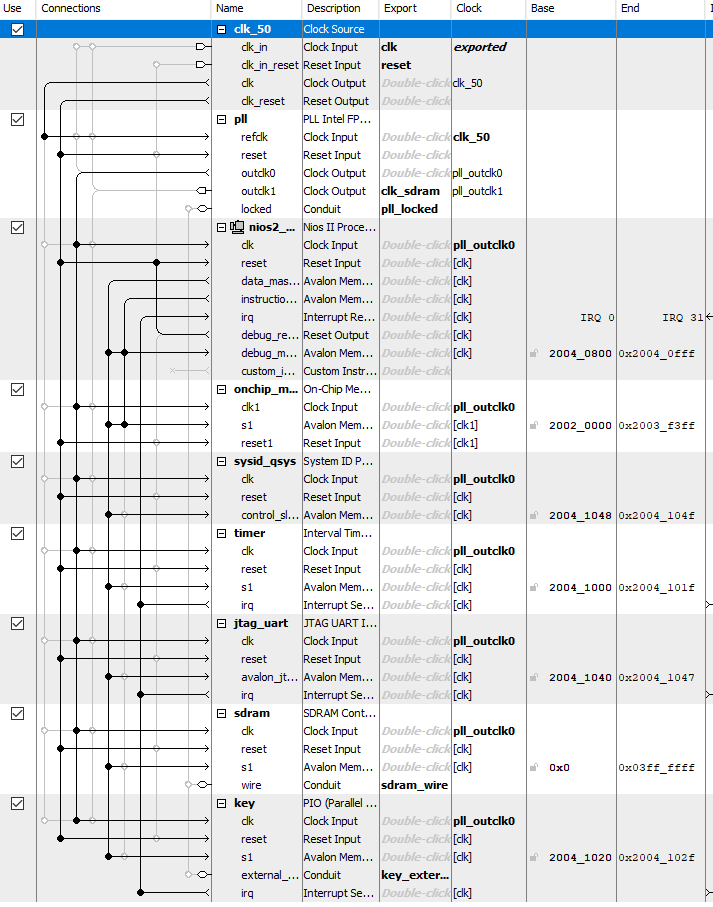
\includegraphics[width=0.7\linewidth]{images/nios_sh_1}
		\caption{Структура построения NIOS ядра}
		\label{fig:niossh1}
	\end{figure}
	
	Ниже приведены компоненты из NIOS ядра и их описания.
	
	\begin{itemize}
		
		\item clk\_50 -- генерация импульса с частотой 50 МГц;
		
		\item pll -- компонент для увеличения частоты и ее синхронизации;
		
		\item nios2 -- процессорное ядро;
		
		\item onchip\_memory -- память выделяемая на кристалле;
		
		\item sysid\_qsys -- идентификатор системы;
		
		\item timer -- таймер или счетчик;
		
		\item jtag\_uart -- модуль для взаимодействия с ПК;
		
		\item sdram -- оперативная память;
		
		\item key -- модуль для работы с кнопками на плате.
		
	\end{itemize}

	Программная часть состоит из двух проектов, проект самой прошивки и проект BSP (Board Support Package).
	BSP генерируется на на основе выбранных параметров для платы.
	Далее необходимо собрать проект с прошивкой, входной точкой является файл main.c, в котором подключаются все необходимые библиотеки для работы с платой.
	
	\subsection{SDRAM Test in Verilog} 
	
	В первом проекте (SDRAM Test in Nios II) использовалось NIOS ядро и вся работа по обработке данных производилась в этом синтезируемом NIOS ядре. При этом программа для ядра (прошивка) писалась на языке C.
	
	Во втором проекте (SDRAM Test in Verilog) синтезируются другие структуры, которые предназначены только для данной задачи. При этом плате не нужна никакая другая программа или прошивка. 
	
	Главное отличие между проектами в том, что в первом используется универсальный NIOS процессор, а во втором способе используются специализированные структуры.
	
	\subsection{5.7 PS/2 Mouse Demonstration} 
	
	Проект состоит из одного модуля, который обрабатывает данные с входа $PS \backslash 2$ и выводит информацию о нажатии клавиш и перемещении мыши.
	

	\section{Самостоятельная работа}
	
	\subsection{Модифицировать пример из раздела 5.4 или 5.5}
	
	Модифицировать пример из раздела 5.4 или 5.5 так, чтобы тестирование памяти было с последовательностью, кодирующей номер группы, номер бригады и ФИО ее участников.
	
	Была модифицирована программа из раздела 5.5, программа в режиме бегущей строки выводит на семисегментные индикаторы необходимую информацию. Результат тестирования представлен на рис. \ref*{fig:wvf1dop}.
	
	\begin{figure}[H]
		\centering
		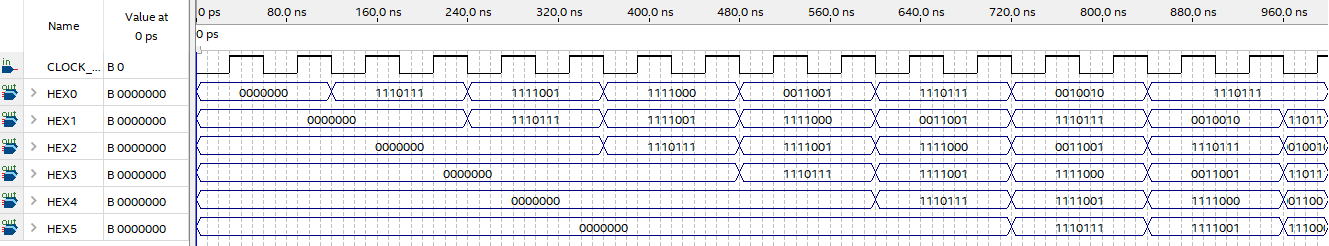
\includegraphics[width=0.9\linewidth]{images/wvf_1_dop}
		\caption{Вейвформа тестирования}
		\label{fig:wvf1dop}
	\end{figure}
	
	
	\subsection{Разработать устройство отображающее на 7-сегментном индикаторе сообщения о выполняемых действиях}
	
	Разработать устройство отображающее на 7-сегментном индикаторе сообщения о выполняемых действиях (раз в 3 с.): ничего не происходит, клик левый (ЛКМ), клик правый (ПКМ), движение вправо/лево и т.д.  
	
	Программа была реализована на языке верилог.
	
	Результаты работы можно наблюдать на вейвформе рис. \ref{fig:wvfdop}. К тестируемому модулю приходят уже обработанные сигналы с мышки, на выход подаются сигналы для семисегментных индикаторов.
	
	\begin{figure}[H]
		\centering
		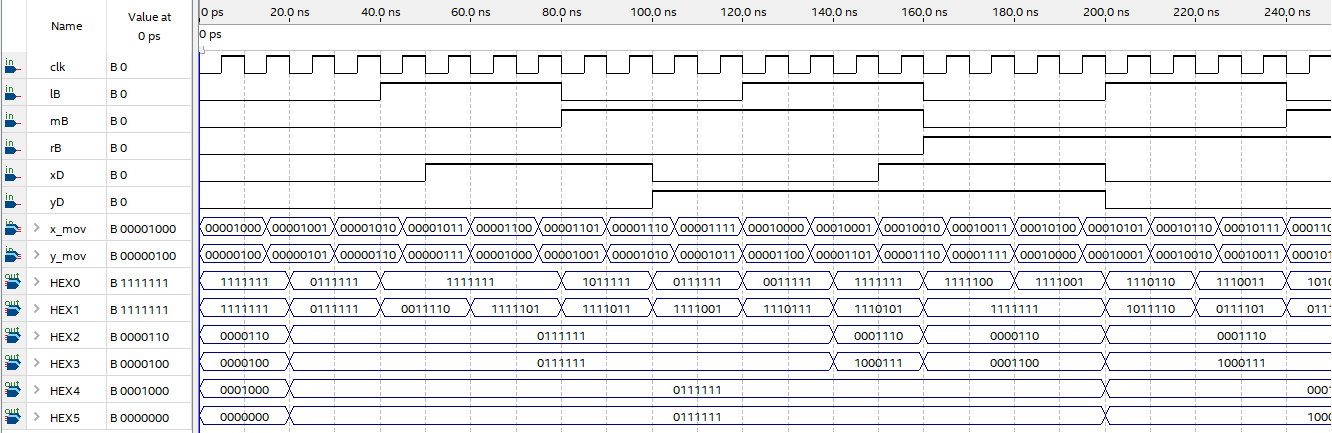
\includegraphics[width=0.9\linewidth]{images/wvf_dop}
		\caption{Вейвформа тестирования модуля выдачи сигналов}
		\label{fig:wvfdop}
	\end{figure}
	
	\section{Выводы по работе}
	
	В ходе работы была изучена работа с оперативной памятью в ПЛИС.
	Был рассмотрен вариант подключения оперативной памяти к NIOS.
	Был получен опыт в написании и анализе кода на языке С.
	Был рассмотрен вариант подключения оперативной памяти при помощи специализированных синтезируемых структур.
	Был получен опыт работы с оперативной памятью при помощи компонентов в $Platform Designer$.
	Был изучен протокол взаимодействия $PS \backslash 2$ .
	Итоговый проект был собран и загружен на плату.
	
	\newpage 
	\renewcommand{\refname}{{\normalsize Список использованных источников}} 
	\centering 
	\begin{thebibliography}{9} 
		\addcontentsline{toc}{section}{\refname} 
		\bibitem{Harris} Хэррис Д. М., Хэррис С. Л. Цифровая схемотехника и архитектура компьютера. – 2015.
	\end{thebibliography}
	
\end{document} % конец документа
